\documentclass[tikz,border=12pt]{standalone}
\usepackage{amsmath}
\usetikzlibrary{arrows.meta,calc,angles,quotes}

\begin{document}
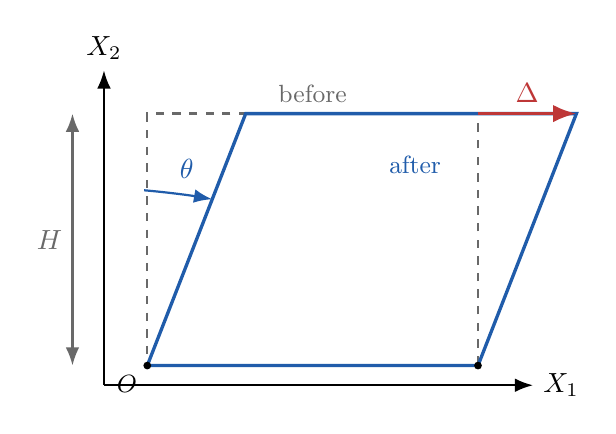
\begin{tikzpicture}[>=Latex,font=\sffamily,thick]
\definecolor{reference}{RGB}{105,105,105}
\definecolor{deformed}{RGB}{32,92,170}
\definecolor{displacement}{RGB}{190,55,55}

\coordinate (A) at (0,0);
\coordinate (B) at (4.2,0);
\coordinate (C) at (4.2,3.2);
\coordinate (D) at (0,3.2);
\coordinate (Cp) at (5.45,3.2);
\coordinate (Dp) at (1.25,3.2);
\coordinate (P) at (0.625,1.6);
\coordinate (Q) at (0.625,2.45);

% Reference and deformed configurations.
\draw[dashed,reference] (A)--(B)--(C)--(D)--cycle;
\draw[deformed,very thick] (A)--(B)--(Cp)--(Dp)--cycle;

% Coordinate directions and dimensions.
\draw[->] (-0.55,-0.25)--(4.9,-0.25) node[right] {$X_1$};
\draw[->] (-0.55,-0.25)--(-0.55,3.75) node[above] {$X_2$};
\draw[<->,reference] (-0.95,0)--(-0.95,3.2)
  node[midway,left] {$H$};
\draw[->,displacement,very thick] (C)--(Cp)
  node[midway,above] {$\Delta$};

% Angle between the X_2 direction and the sheared vertical material line.
% \draw[dashed,reference] (P)--(Q);
\draw[deformed,<-] (P) ++(68.7:0.55) arc (80:85:10);
\node[deformed] at (0.5,2.5) {$\theta$};

\fill (A) circle (1.4pt) node[below left,font=\small] {$O$};
\fill (B) circle (1.4pt);
\node[reference,font=\small] at (2.1,3.45) {before};
\node[deformed,font=\small] at (3.4,2.55) {after};
\end{tikzpicture}
\end{document}